\documentclass[10pt,twoside]{report}
\usepackage{url}
\usepackage{graphicx}
\usepackage{caption}
\usepackage{subcaption}
\usepackage{listings}
\usepackage{xcolor}
\usepackage{framed}
\usepackage{pgfplotstable}
\usepackage{pgfplots}
\lstset{language=Python, keywordstyle=\color{blue}\bfseries, }
\usepackage{amsmath}

\newcommand{\cmnt}[1]{}
%\newcommand{\Transp}[2]{\ensuremath{Tranp(#1,#2)}}
%\newcommand{\Antloc}[2]{\ensuremath{Antloc(#1,#2)}
%\newcommand{\Xcomp}[2]{\ensuremath{Xcomp(#1,#2)}}
%\newcommand{\Eval}[2]{\ensuremath{eval(#1,#2)}}
%\newcommand{\Mod}[2]{\ensuremath{mod(#1,#2)}}

\newcommand{\Alpha}[1]{\ensuremath{\alpha(#1)}}
\newcommand{\Beta}[1]{\ensuremath{\beta(#1)}}
\newcommand{\myGamma}[1]{\ensuremath{\gamma(#1)}}
\newcommand{\myin}[1]{\texttt{In(#1)}}
\newcommand{\myout}[1]{\texttt{Out(#1)}}
\newcommand{\antin}[1]{\texttt{Antin(#1)}}
\newcommand{\antout}[1]{\texttt{Antout(#1)}}
\newcommand{\antloc}[1]{\texttt{Antloc(#1)}}
\newcommand{\transp}[1]{\texttt{Tranp(#1)}}
\newcommand{\xcomp}[1]{\texttt{Xcomp(#1)}}
\newcommand{\availin}[1]{\texttt{Availin(#1)}}
\newcommand{\availout}[1]{\texttt{Availout(#1)}}
\newcommand{\earlin}[1]{\texttt{Earliestin(#1)}}
\newcommand{\earlout}[1]{\texttt{Earliestout(#1)}}
\newcommand{\delayin}[1]{\texttt{Delayin(#1)}}
\newcommand{\delayout}[1]{\texttt{Delayout(#1)}}
\newcommand{\latestin}[1]{\texttt{Latestin(#1)}}
\newcommand{\latestout}[1]{\texttt{Latestout(#1)}}
\newcommand{\isoin}[1]{\texttt{Isolatedin(#1)}}
\newcommand{\isoout}[1]{\texttt{Isolatedout(#1)}}
\newcommand{\insertin}[1]{\texttt{Insertin(#1)}}
\newcommand{\insertout}[1]{\texttt{Insertout(#1)}}
\newcommand{\replacein}[1]{\texttt{Replacein(#1)}}
\newcommand{\replaceout}[1]{\texttt{Replaceout(#1)}}
\pagestyle{myheadings}

\bibliographystyle{siam}

\addtolength{\textwidth}{1.00in}
\addtolength{\textheight}{1.00in}
\addtolength{\evensidemargin}{-1.00in}
\addtolength{\oddsidemargin}{-0.00in}
\addtolength{\topmargin}{-.50in}

\hyphenation{in-de-pen-dent}


\title{\textbf{Partial Redundancy Elimination using Lazy Code Motion}}

\author{Sandeep Dasgupta\thanks{Electronic address:
\texttt{sdasgup3@illinois.edu}} \qquad Tanmay Gangwani\thanks{Electronic
address: \texttt{gangwan2@illinois.edu}}}

\begin{document}
\begin{titlepage}
\thispagestyle{empty}
\maketitle
\pagebreak
\end{titlepage}

\begin{flushleft}
\textbf{\Large{Summary}}
\end{flushleft}

Having identified the computationally and lifetime optimal placement points
  previously, we spent the bulk of the time in this phase in the following items:
  \begin{enumerate}
    \item Adding code to insert and replace expressions 
    \item Handling loop invariant code motion 
    \item Building up the testing infrastructure and initial testing. 
   \end{enumerate} 
Below we detail each of these steps.

\begin{flushleft}
\textbf{\Large{Insert and Replace}}
\end{flushleft}
To maintain compatibility with SSA, we perform insertion and replacement
  through memory and re-run the \emph{mem2reg} pass after our PRE pass to convert the
  newly created load and store instructions to register operations. Following
  are the major points:
\begin{itemize}  
  \item Assign stack space \emph{(allocas)} at the beginning of the
  function for all the expressions that need movement
  \item At insertion point,
           compute the expression and save the value to the stack slot assigned to the
             expression 
  \item At replacement point, load from the correct stack
             slot, replace all uses of the original expression with the load
             instruction, and delete the original expression
  \item \emph{mem2reg} converts stack operations to register operations and introduces the 
             necessary ${\Phi}$ instructions
\end{itemize}  

Working on same example (with some added complexity) as that in our phase-1 report, we show in Figure\ref{fig:1}
and Figure\ref{fig:2}, the optimizations performed by our PRE pass. The intention here is to
  show how our version of PRE performed on the computations $a + b$ \& $a < b$;


\begin{figure}[htbp]
  \begin{center}
     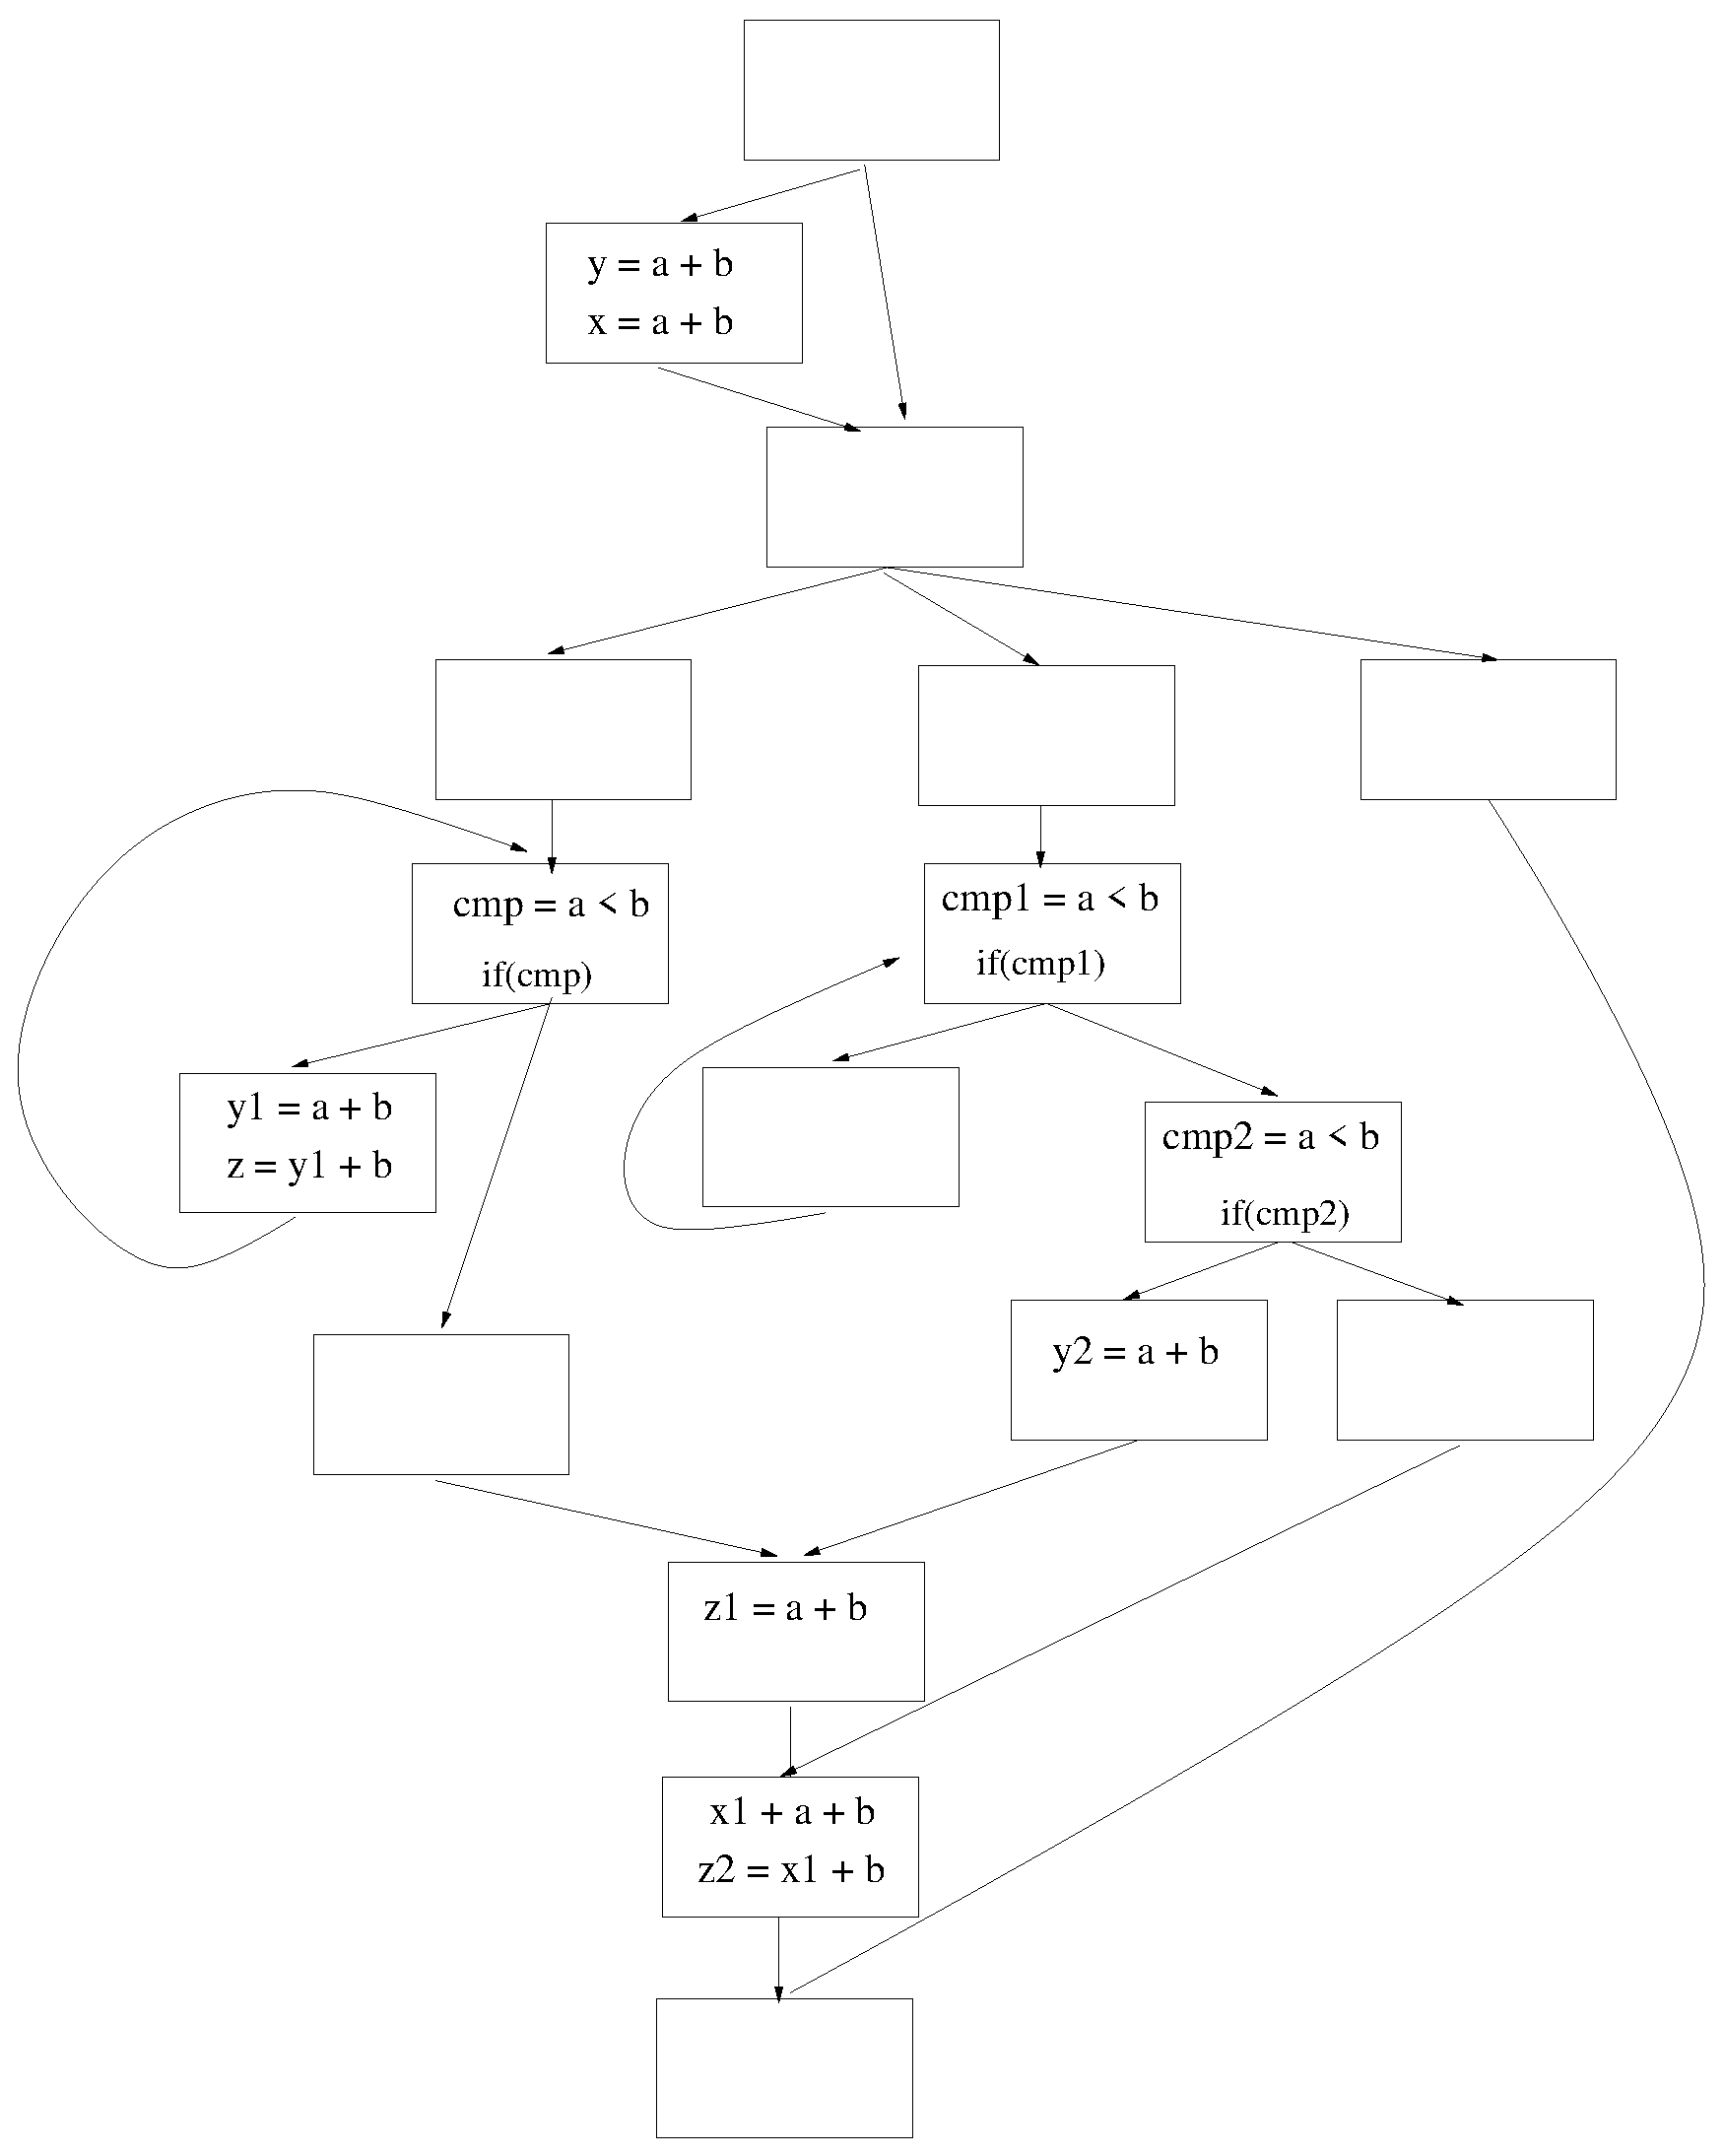
\includegraphics[scale=0.4]{1} 
  \end{center}
  \caption{A motivating example}
    \label{fig:1} 
\end{figure}

\begin{figure}[htbp]
  \begin{center}
     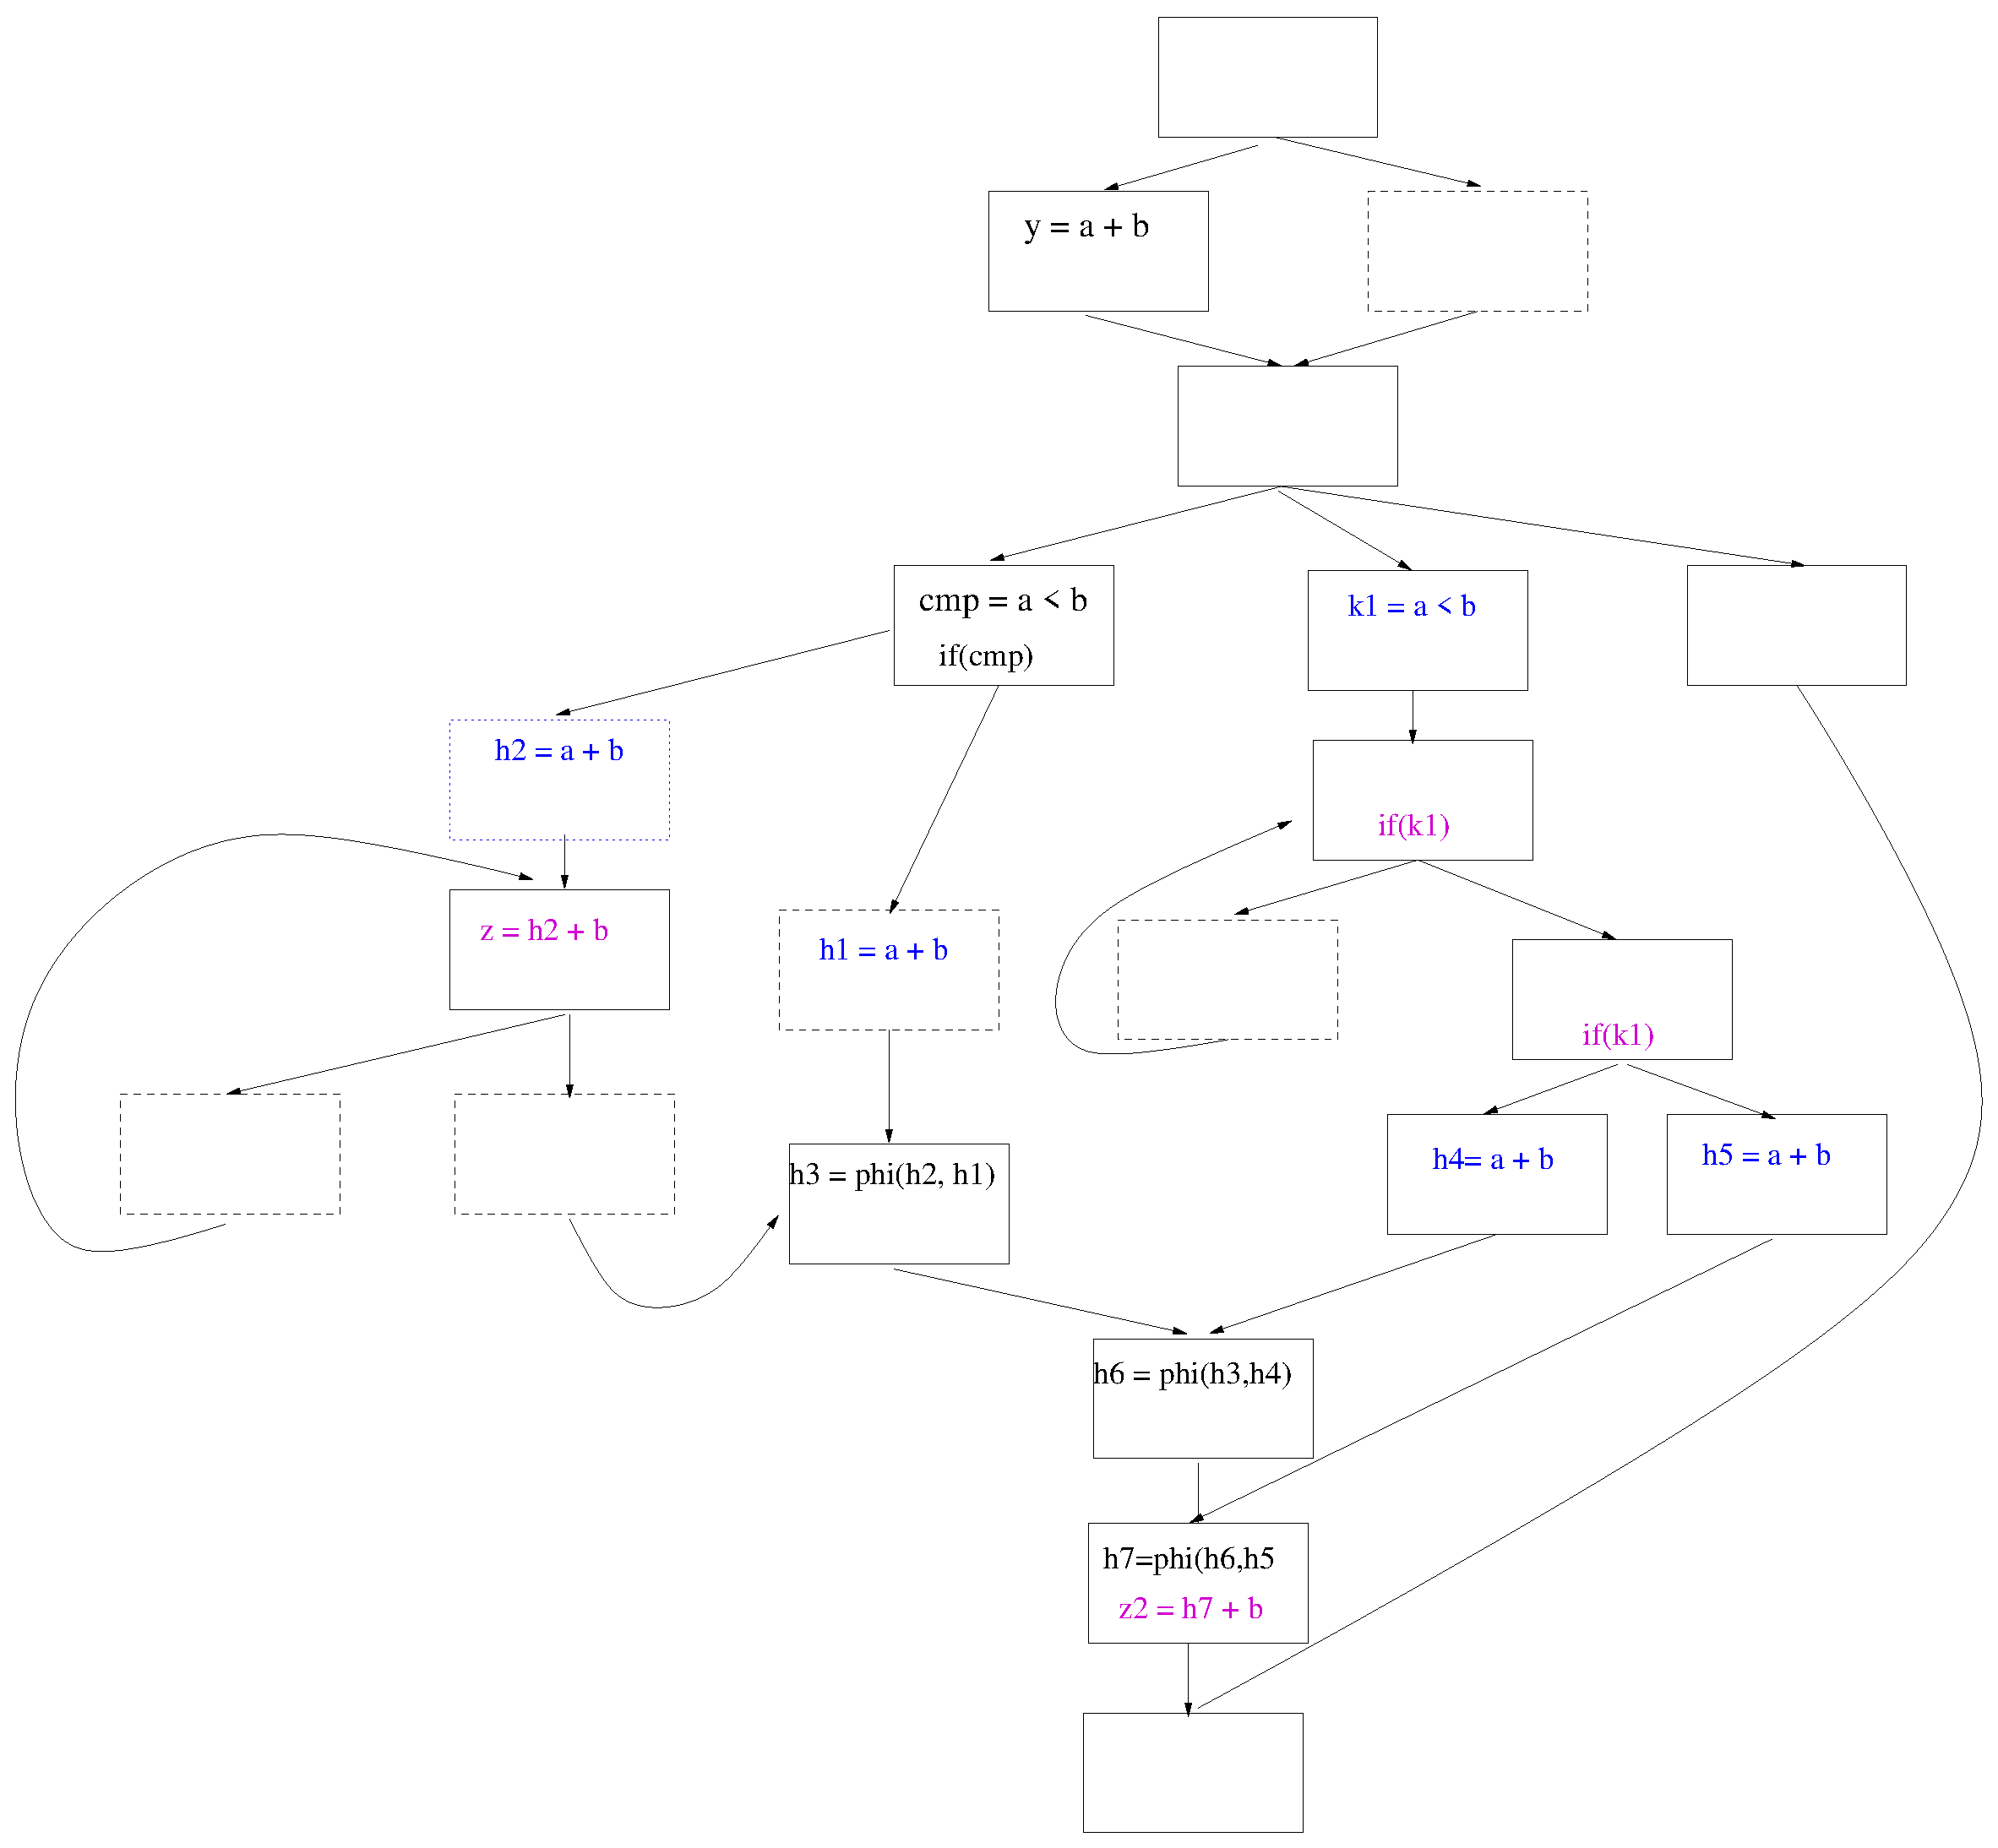
\includegraphics[scale=0.4]{2} 
  \end{center}
  \caption{Lazy code motion transformation on computations $a + b$ \& $a < b$.
    Dotted boxed denote critical edges. Blue dotted boxes are the ones inserted by loop
      rotate. PRE can insert the computations in these places. Inserted statements are marked
      \textcolor{blue}{blue} and replaced ones with \textcolor{magenta}{magenta} } 

  \label{fig:2} 
  \end{figure}

\cmnt{    
One point about the insertion
  step is worth mentioning. Suppose that an expression, with value number vn,
       is to be inserted in a basic block. Although our algorithm can handle
         all cases, for simplicity, assume that the insertion point is the end
         of the basic block. To insert the expression we scan the list of the
         expressions in the whole function which have the same value number vn.
         We then clone one of these expressions (called provider) and place at
         the end of the basic block. The trivial case is when the the provider
         is available in the same basic block. If however, the provider comes
         from another basic block, then we need to ensure that the operands of
         the provider dominate the basic block where we wish to insert the
         expression in. Not being able to find a suitable provider is the only
         case where we override the suggestion of the data flow analysis and
         not do PRE for that expression only. PRE for other expressions
         proceeds as usual. Our initial testing suggests that this is a very
         rare occurrence. Fig [] is a motivating example. We would quantify
         this for real applications in our final report.  
}

\begin{flushleft}
\textbf{\Large{Loop Invariant Code Motion}}
\end{flushleft}
We first address a question raised in the phase-1 report. We had previously
mentioned that to optimize for space and time, we provide a bit vector slot only to
value numbers which have more than one expression linked to them. With this,
      however, we could miss opportunities for loop invariant code motion. As a
      solution, we extend the bit vector to include value numbers which have
      only a single expression linked to them but only if the expression is
      inside a loop. Note that we still exclude the cases where the expression
      is not part of a loop, and expect reasonable space and time savings.  

      The second issue we resolved with respect to loop invariant code motion was 
      checking for zero-trip loops. Our PRE algorithm would move the loop invariant
      computations to the loop pre-header only if placement in the loop pre-header is 
      anticipatible. Such a pre-header is always available for \emph{do-while} loops, 
      but not for \emph{while} and \emph{for} loops. Hence, a modification is required
      to the structure of \emph{while} and \emph{for} loops which peels off the first
      iteration of the loop, protected by the loop condition. This alteration provides 
      PRE with a suitable loop pre-header to hoist loop independent computations to.
      In Figure \ref{fig:3} we show the CFG changes. Fortunately, we were able to 
      achieve this effect using an existing LLVM pass \emph{-loop-rotate} rather than
      having to write it ourselves.

\begin{figure}[htbp]
  \begin{center}
     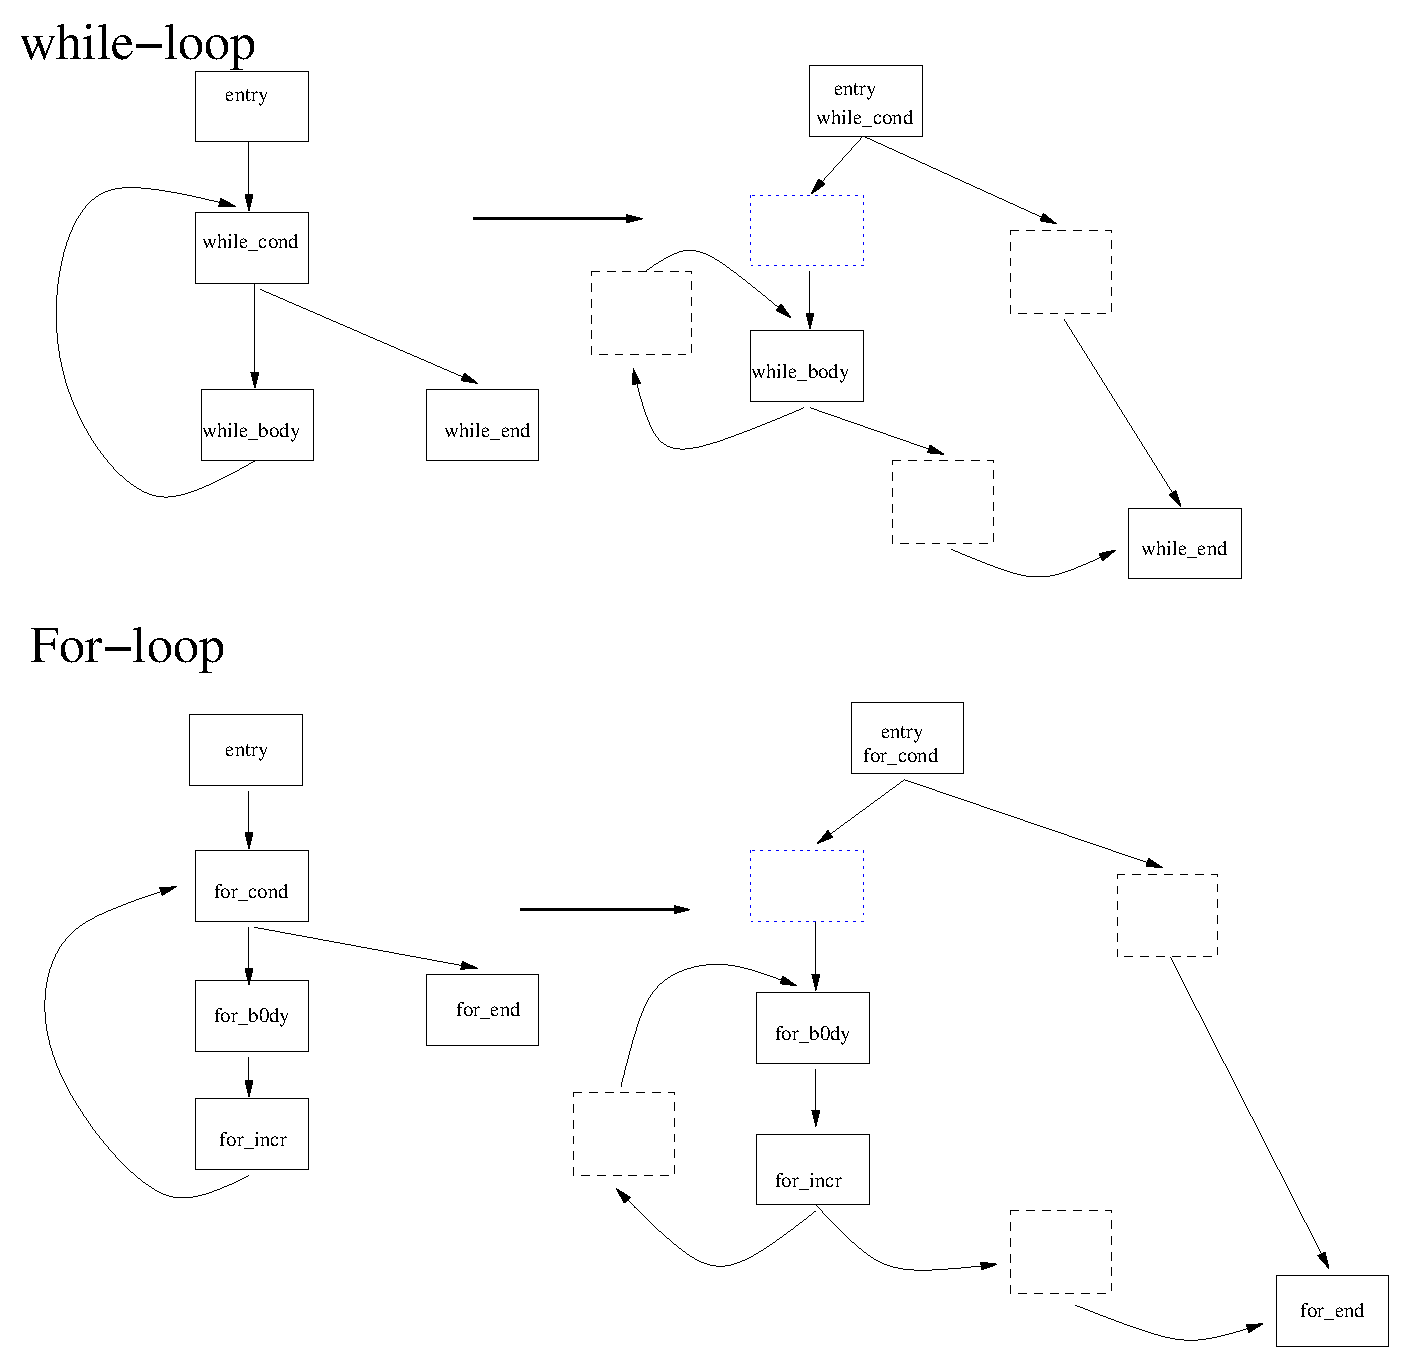
\includegraphics[scale=0.5]{3} 
  \end{center}
  \caption{Loop transformations done by \emph{-loop-rotate}. \emph{do-while}
    loops remain unaffected. Blue dotted boxes are the ones inserted by loop
      rotate. PRE can insert the computations in these places.}

  \label{fig:3} 
  \end{figure}


\newpage  
\begin{flushleft}
\textbf{\Large{Testing}}
\end{flushleft}

Apart from the small test cases which we created in phase-1, we have been able to 
successfully test our PRE pass on real codes from the LLVM test-suite. Specifically, we have
completed the testing for 75 benchmarks from LLVM single-source package \emph{"test-suite/SingleSource/Benchmarks/"} for correctness and performance. Correctness is checked by
comparing the output of the binary optimized with our PRE pass with the reference output 
provided along with benchmarks. All benchmarks pass the correctness test. For performance, 
we compile the codes with and without the PRE pass and take the ratio of the run-times on 
the hardware. Figure 4 shows the S-curve for performance. For 55/75 benchmarks, our pass improves 
the run time by varying amounts (upto 67\%). Performance drops for few benchmarks, but the degradation is bound by 8\%.

Apart from measured runtime on the hardware, another metric to quantify the
effects of our optimization pass is the dynamic instruction count. We use Pin
(dynamic binary instrumentation tool) from Intel for this purpose. We have
written a very simple Pintool to dump the dynamic instruction count of each
type of instruction. We would present supporting data from Pin our final
report.
%\pgfplotstabletypeset{data.dat}

\begin{figure}
\begin{center}
\begin{tikzpicture}
\begin{axis}[
  xlabel=Benchmark number,
  ylabel=Base Time/ PRE Time,
  ymax=1.7, ymin=0.8, xmax=80,
  x tick label style={black},
  grid=both,xmajorgrids=false,
  ]
\addplot table [y=T, x=N]{data.dat};
\end{axis}
\end{tikzpicture}
\end{center}
\label{fig:4}
\caption{S-curve for performance improvements over Baseline (no PRE)}
\end{figure}

\begin{flushleft}
\textbf{\Large{{Conclustion and Future Work }}}
\end{flushleft} 
In this phase, we were able to code the missing pieces of our PRE algorithm,
   thereby achieving full functionality of the project. The highlights were the
   insert-replace algorithm, LICM improvements, and fixes for numerous bugs
   which surfaced during testing on the LLVM single-source package. We have
   written scripts to automate the testing, and this would speed up work for
   the final phase. \\ 
   The S-curve in this report (Figure 4)
   presents improvements with respect to the baseline (no PRE pass) for
   single-source package. We would like to evaluate the cases where our pass
   degrades performance compared to baseline. In our final report, we plan to
   include similar curves for benchamarks from the LLVM multi-source package as
   well as the SPEC 2006 suite. Also, we would include S-curves to compare the
   effectiveness of our PRE pass with the LLVM GVN-PRE pass. For extreme
   outliers, we hope to present supporting data to reason about the performance
   change. Pin tool analysis and the statistics dumped by our PRE pass would be
   used for this.

  
\end{document}
